% simple.tex 

\documentclass{article}

\usepackage{times}
\usepackage{amssymb, amsmath, amsthm}
\usepackage{graphicx}
\usepackage[margin=1in]{geometry}

\begin{document}

\title{MTH 338 Homework}
\author{Philip Warton}
\date{\today}
\maketitle
\section{SAS in Elliptic Geometry}
To verify that two triangles with two congruent sides and a congruent angle between them will be entirely congruent in Elliptic geometry, we will construct two triangles with such properties and check the remaining side and angles for congruency on the Klein Disk. Let $A,B,C$ be points on the Klein Disk. Construct the lines $\overleftrightarrow{AB}, \overleftrightarrow{BC}, \overleftrightarrow{CA}$, who form a triangle. One can construct a circle $c_1$ centered at $B$ that intersects $A$, and a circle $c_2$ centered at $B$ that intersects $C$. The circle $c_1$ intersects the line $\overleftrightarrow{AB}$ at point $A$ and at another point which we will label $D$. Similarly we can label the other intersection point between $c_2$ and $\overleftrightarrow{BC}$ as $E$. We have constructed the triangle $\vartriangle EBD$ such that it has two sides and the angle in between them congruent to the triangle $\vartriangle CBA$, as seen in $\fbox{Figure 1}$. Measuring the remaining sides and angles it can be seen that they too are congruent, as demonstrated in $\fbox{Figure 2}$.
\begin{figure}
	\caption{Two triangles on the Klein disk with congruent SAS}
	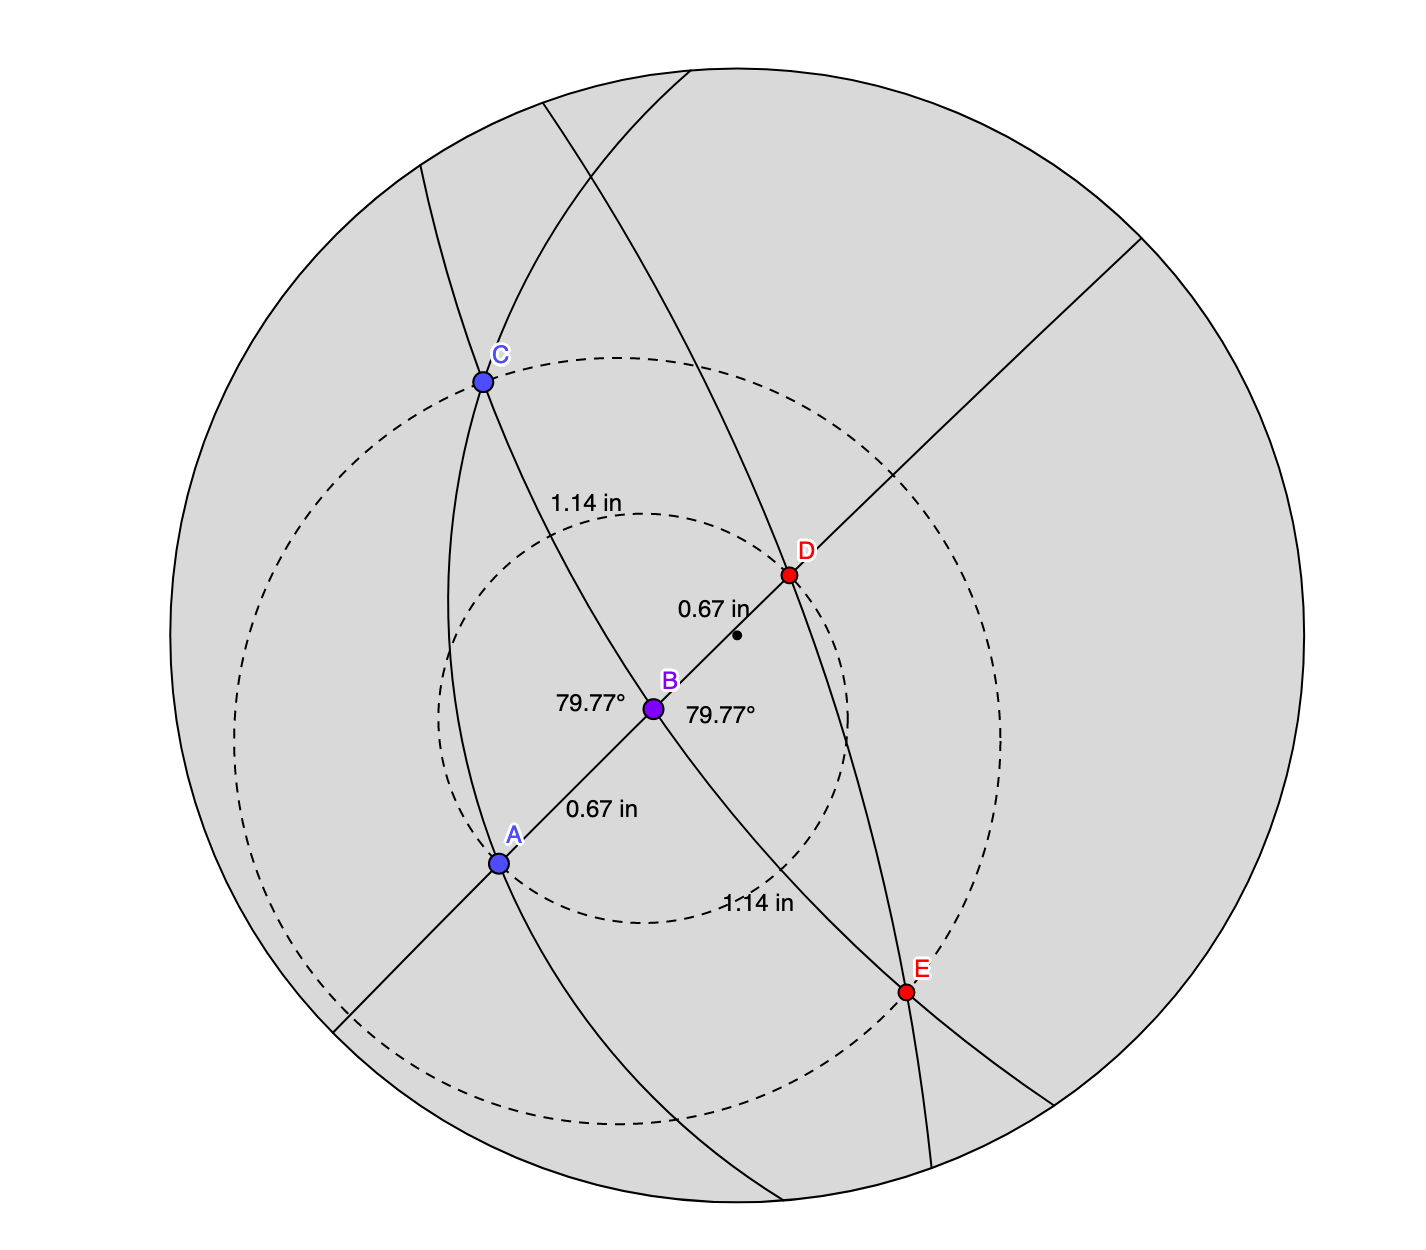
\includegraphics[scale=0.4]{/Users/philip/Documents/OSU/Math/338/SAS_klein}
\end{figure}
\begin{figure}
	\caption{Verifying complete congruence among triangles}
	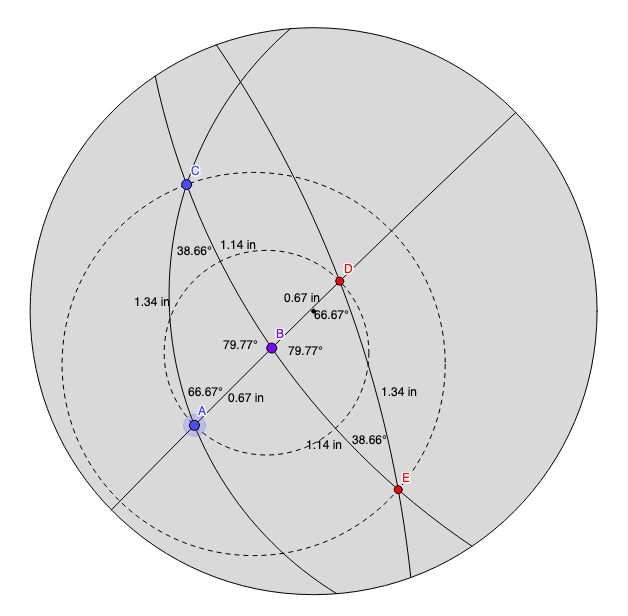
\includegraphics[scale=0.4]{/Users/philip/Documents/OSU/Math/338/SAS_klein_2}
\end{figure}
\section{Circles in the Klein Disk}
	To construct a complete circle on the Klein Disk which intersects the equator exactly twice, let us determine what is not valid. If we draw a diameter, equivalent to a great circle on a sphere, then we get a line that is a circle, that intersects the antipodal points. However, since those two antipodal points are consider one point, this is not a valid solution. If we choose the outer rim, we have a circle that intersects the equator at infinitely many points. Therefore we must construct some other circle. Choose a point (not the center) on the Klein disk, and let that be the center of our circle. 

For some interval $(0, x)$, if the radius of our circle is within this interval the circle will not intersect the equator at all. Therefore, when the radius is exactly equal to $x$, the circle will intertersect the equator exactly once. We must choose a radius that is greater than this distance $x$ so that We have two points of intersection between our circle and the equator. We must continue the circle on the opposite part of the Klein disk by constructing three diameters, one through our initial point, and two through our intersection points. The antipodal points to the intersection are the same points and must intersect the circle still. If we extend the diameter through our initial point and the origin outside of the disk, then there is only one circle which intersects our two antipodal points with the same radius as the first circle we drew that has its center on the extended diamater. See $\fbox{Figure 3}$.

\begin{figure}
	\caption{Klein Disk circle intersecting the equator exactly twice (there is an error in that the radii do not appear exactly equal)}
	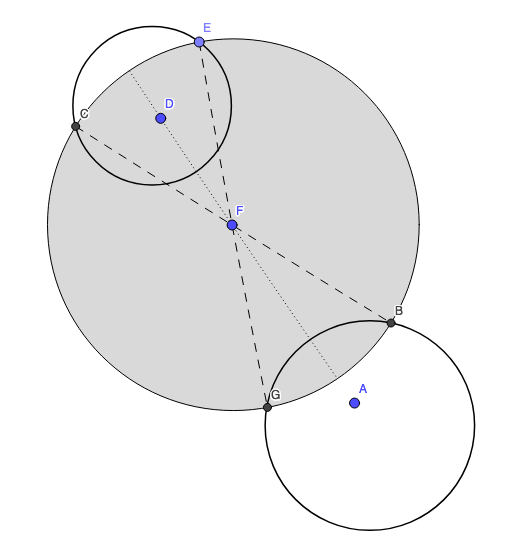
\includegraphics[scale=.7]{/Users/philip/Documents/OSU/Math/338/circles_klein}
\end{figure}
\end{document}